\chapter{Bedürfnisanalyse}

Im Kapitel der Bedürfnisanalyse werden Anwendungsfälle ermittelt welche mit Smartwatches abgedeckt werden können. Zusätzlich wird eine Bedarfsanalyse durchgeführt für Applikationen welche in Verbindung zur siot.net Plattform stehen.
\section{Smartwatch Applikationen}
\subsection{Gesundheit}
Im Gesundheitssektor gibt es einige Anwendungsfälle welche mit einer smarten Uhr abgedeckt werden können.

Eine Smartwatch bietet die Möglichkeit sich zu überwachen. Da die Computeruhr mit vielen Sensoren, wie z.B. Bewegungsensor oder Herzfrequenzmesser, ausgerüstet ist, hat sie die Möglichkeit den Träger sehr genau zu analysieren.

Bei einem Sturz des Benutzers kann ein Alarm ausgelöst werden. Dieser würde in erster Instanz eine positive Gesundheitsbericht des Anwenders verlangen. Diese Bestätigung sollte in einem definierten Zeitrahmen statt finden. Falls dies nicht ausgeführt wird und die Uhr keine Bewegung registriert, kann ein Alarm an eine Vertrauensperson oder gar ein Notruf ausgelöst werden. Dieser Notruf kann wichtigen Daten angereichert werden, wie z.B. Pulsdaten und die GPS Koordinaten. Statt des Sturzes kann hier der Auslöser des Alarmes auch ein zu tiefer oder gar kein Puls sein.

Ein weiterer nützlicher Use-Case ist, Alarme von Patienten im Spital. Hier kann das Pflegepersonal mit Smartwatches, Patientenalarme erhalten. Die Alarme sollten möglichst nur empfangen werden, wenn der Patient in der nähe des Patienten sich befindet. Wenn mehrere Pfleger/innen benachrichtigt werden, kann eine Pflegeperson den Alarm bestätigen und die Verantwortung für den Patient übernehmen, so können Doppelspurigkeiten vermieden werden.

\subsection{Smart Home}
Für die Fernbedienung von Geräten im Haus oder Wohnung eignet sich die Smartwatch gut. Mit eingebauten Touchscreen und Vibrationsmotor, haben die kleinen Handgelenkrechner die Möglichkeit Informationen visuell wie taktil an die Person zu bringen.

Geräte im Haushalt können überwacht werden. Dies hilft Gefahren abzuwenden. Wenn eine Herdplatt noch läuft kann ein Alarm ausgelöst werden und es kann gleich mit der Uhr reagiert werden und die Platte ausschalten.

Für jeden einen Mehrwert gibt die Funktion Licht vom Handgelenk zu bedienen. Es ist bequem das Zimmer zu beleuchten ohne zum Lichtschalter gehen zu müssen. Dimmen mit dem Touchscreen und terminierte Lichtsteuerung. Auch eine automatische Beleuchtung durch erkennen der Helligekeit im Raum ist eine Funktion mit hohem Potenzial.

Ein weiterer Anwendungsfall ist die Waschmaschine. Die Restzeit des Waschgangs kann auf den Bildschirm angezeigt werden und wenn er beendet ist, wird der Träger mit einem Vibrationsimpuls notifiziert.

Desweiteren ist das Fernbedienen von allen Multimediageräten vom Handgelenk sehr praktisch. Es genügt eine Uhr und braucht nicht mehr viele verschiedene proprietäre Steuerungen. Dies wird heute bereits mit Smartphone Apps praktiziert. Mit Sprachsteuerung können Personen mit eingeschränkter Sehkraft die Uhr verwenden.

\subsection{Sport}
Heute werden Smartwatches hauptsächlich als Fitnesstracker verwendet\footnote{vgl. Studienband Smartwatch Umfrage eResult, Ausgabe: Juni 2015}. Das Praktische an den Uhren unter den Wearables ist, dass diese nicht nur für zum Sport treiben gekauft werden muss. Hier erhält der Endkunde ein Gerät für den Alltag und die Freizeit.

Im Sportbereich kann mit den vorhandenen Sensoren viele verschiedene Werte ermittelt und analysiert werden. Mit den nötigen Voreinstellungen, wie Körpermasse, Schrittlänge, Alter und Geschlecht, ist es möglich Bewegungsdaten genau aufzuzeichnen. Mit den Daten können für den Anwender interessante Informationen berechnet werden. Für Hobbysportler meist relevante Berechnungen sind Zeit, Schritte, Geschwindigkeit und Kalorienverbrauch. Für erfahrene Sportler verbessern ihre Fähigkeiten durch betrachten von Auswertungen der Körperbelastungen, z.B. Beschleunigung, Stärke, Drehmoment und weitere.

\subsection{Ortsbezogen}
Applikationen welche umgebungsorientiert arbeiten, sind geeignete Kandidaten für Smartwatches. Durch die permanente Anzeige am Handgelenk, können schnell ändernde Daten dauerhaft im Auge behalten werden.

Ein Anwendungsfall ist, das Smartphone zu überwachen. Die Uhr kann den Träger informieren, wenn das Sichtbarkeitsumfeld vom Mobiltelefon und des tragbaren Rechners sich nicht mehr überschneiden, was bedeuten würde die Geräte entkoppeln sich voneinander.

Die gleiche Methode bietet sich an, Personen mit Smartwatches in der Nähe zu scannen. Diese Funktion kann bei Partnervermittlungsapplikationen effektiv eingesetzt werden. Durch den vorhandenen Touchscreen können potenzielle Datingpartner angezeigt und kontaktiert werden. In der schnelllebigen Welt sind sich schnell erschliessende Kontakte sehr willkommen.

Ein weiterer Punkt ist Geofencing. Mit Geofencing werden automatische Aktionen eingeleitet. Diese geschehen sobald bestimmte geografische Grenzen überschritten werden. Über eine Ortung des Gerätes kann ermittelt werden ob dieses sich in einer Geofencing Zone befindet. Mit Smartwatches kann dies effektiver genutzt werden, da durch den immer sichtbaren Bildschirm, die ortsrelevanten Daten ohne Zeitverlust angezeigt.\\
Eine Geofencing Anwendung wäre Sehenswürdigkeiten präsentieren. Eine App welche für jede Sehenswürdigkeit eine Geofencing Zone errichtet oder kennt und jeweils die Auskunft des Objektes darstellt.

Die Indoornavigation ist ein Bedürfnis welches mit Smartwatche nicht gelöst jedoch erweitern kann. In Zusammenarbeit mit Beacons/Eddystones und/oder Access Points können die Standorte von Smartwatchträger, im inneren von Räumen, ermittelt werden. Beacons und Eddystones sind Sender/Empfänger welche auf Bluetooth Low Energy (BLE, Bluetooth 4.0 oder  Bluetooth Smart).\\
Grossfirmen können eine grossen Nutzen aus dieser Technologiekombination schöpfen. Die Mitarbeiter ihren Standort preisgeben, damit diese gefunden werden können ohne zu suchen. Es können Geofencing Zonen definiert werden um die Zeiterfassung zu automatisieren. Beim eintretten, des geografisch definierten Bereichs, welcher zu Arbeitszone gehört, wird Arbeitszeit erfasst. Verlässt der Mitarbeiter diesen Teil des Gebäudes, wird die Arbeitszeiterfassung gestoppt.\\
Zusätzlich kann das Problem mit den Shared-Desk Arbeitsplätzen kann gelöst werden. Bei diesem Arbeitsplatzmodell richtet sich der Mitarbeiter jeden Tag an dem Ort ein wo es einen freien Platz hat. Da dieser nicht im vorherein weiss wo der nächste freie Platz ist, führt dies zu Verlusten, wenn Zeit benötigt wird um einen Arbeitsplatz zu suchen. Mit der Smartwatch ausgetattet, ist der Angestellte in der Lage, vorgängig einen freien Arbeitsplatz zu reservieren und sich anzumelden, beim erreichen des Schreibtisches.
\newpage

\subsection{Authentifikation}
Im Authentifikationssektor gibt es einige Bedürfnisse welche mit Smartwatches gedeckt werden können

Türen entrigeln mit der Smartwatch ist ein geeigneter Anwendungsfall. Heute benutzen die meisten Automobilhersteller ein Keyless System für ihre Fahrzeuge. Mit diesen Systemen hat der Fahrer nur ein Sender/Empfänger, mit einem einzigartigem Zertifikat, welches sich mit dem Fahrzeuges korreliert. Türen werden geöffnet und Motoren werden gestartet, diese Funktion könnte auch die Smartwatch übernehmen. Damit hätte der Fahrzeugbesitzer ein Utensil weniger zu mitzutragen.

Die intelligente Uhr hat das Potenzial Personalausweise zu ersetzen. Wie bereits im Abschnitt Ortsbezogen erwähnt kann es zur Zeiterfassung genutzt werden. Das heisst Mitarbeiter muss nicht mehr an die Zeiterfassungsleser.

\subsection{Finanztechnologie - FinTech}
Die Möglichkeit zu haben mit der Uhr Zahlunge zu authorisieren ist ein Bedürfnis, welches erschaffen werden kann. Denn es scheint praktisch einzukaufen gehen ohne das Portmonee dabei zu haben. Es sind Lösungen vorhanden, welche mit Smartphones funktionieren {(Abbildung 4.1 Apple Pay/Google Wallet/TWINT)}. Mit der Lancierung der Apple Watch, erreichte die erste Smartwatch mit einer Zahlfunktion, sie unterstützt Apple Pay, den Markt.

\section{Smartwatch Applikationen für siot.net}
Die siot.net Plattform bietet sich bestens als Kommunikationsschnittstelle an für die Applikationen, welche im vorherigen Abschnitt ermittelt wurden. Die meisten Bedürfnisse verlangen irgendeine Art von Kommunikation. Ob es nur übermitteln der Sensordaten ist oder die Abfrage eines Sicherheitstokens ist, die siot.net Plattform erlaubt sämtliche Informationen über eine Schnittstelle auszutauschen. Damit es einfacher wird sollten möglichst viele oder besser alle Geräte, welche miteinander kommunizieren sollen, an die siot.net Plattform angebunden werden.
\begin{figure}[h]
  \centering
  \includegraphics[scale=0.2]{98_Bilder/04_Anwendungen/APay_GWallet_PFTwint.png}
  \caption[Mobile Zahlungslösungen: Apple Pay, Google Wallet und TWINT powered by PostFinance]{Bekannte Zahlungslösunge für Smartphone: Apple Pay, Google Wallet und TWINT powered by PostFinance}
  \footnotesize \url{http://www.apple.com/apple-pay/} \url{https://wallet.google.com/} \url{http://www.twint.ch/ueber_uns/medien/}, 04.12.2015
\end{figure}

\subsection{siot.net Gateway Library}
Um Verknüpfungen individueller Applikationen von Smartwatches oder auch Smartphones mit der Plattform zu ermöglichen, sollte es eine generische Biblithek geben. Diese sollte eine einfache Schnittstelle implementieren, welche Applikation an die siot.net Plattform anbindet. Eine automatische Erkennung aller Sensoren vereinfacht die Entwicklung von Apps welche zum siot.net IoT-Center kommunizieren wollen.

\subsection{siot.net Sensorcenter}
Jedes Android Gerät kann mit den eingebauten Sensoren hervoragend als Sensorstation dienen. Um die Vielzahl von Sensor in Eigenregie zu im siot.net zu manifestieren und Sensordaten preiszugeben, sollte es ein App geben mit einer möglichst eifachen grafischen Benutzeroberfläche.

\subsection{siot.net Dashboard App}
Um Auswertung und Darstellung von den Daten zu habe, gibt es von siot.net bereits eine Dashboard Webapplikation. Um diese Funktionen einem Smartphone, in einer kompakten Form, zur Verfügung zu stellen, eignet sich eine App. Diese App sollte von Vorteil durch den Benutzer konfigurierbar sein.

\subsection{Herzfrequenz Überwachung}
Vielen Personen, welche ihren Puls im Griff haben wollen, leichte gesundheitliche Probleme haben oder jemanden alarmieren will bei Unregelmässigkeiten bei der Herzfrequenz, würden eine Herzfrequenz Überwachung begrüssen. Diese Anwendungfälle kann mit einer Smartwatch und der siot.net Plattform abgedeckt werden.

\subsection{Steuerung von Modellen}
Modellbau und Smartphones ist keine Weltneuheit, es wird schon rege verwendet, wie bei der Parrot bebop Drohne\footnote{Quelle: \url{https://s.gravis.de/p/z1/parrot-bebop-drone-kamera-drohne-fuer-smartphones-tablets-gps-blau_z1.jpg}, Stand: 04.12.2015 } (siehe Abbildung 4.4). Das Potenzial mit einer Steuerung (Smartphone oder Smartwatch) mehrere Modelle simultan zu steuern, scheint jedoch noch nicht im grossen Stile abgerufen zu werden.
Mit der Anbindung von Modellen an das Internet der Dinge, zusätzlich gekoppelt mit einem einer smarten Steuerungseinheit, kann dieses Bedürfnis abgedeckt werden. Die siot.net Umgebung bietet dazu eine günstige Ausgangslage.
\begin{figure}[h]
  \centering
  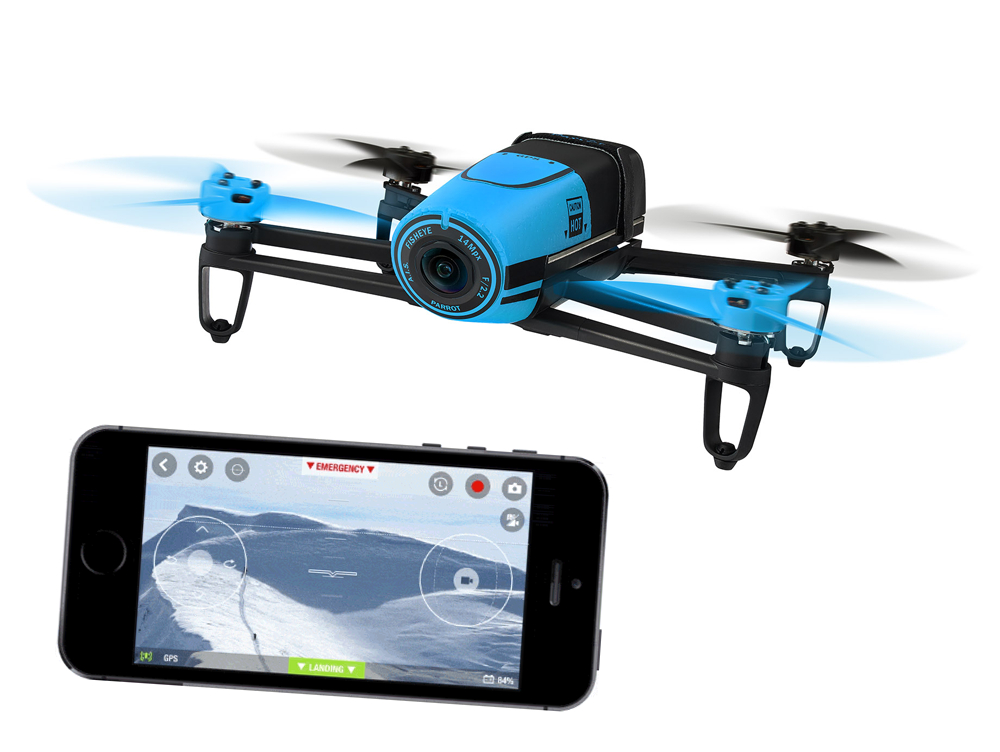
\includegraphics[scale=1]{98_Bilder/04_Anwendungen/parrotdrone}
  \caption[Smartphone gesteuerte Drohne: Parrot bebop]{Parrot bietet Drohnen an, welche mit dem Smartphone gesteuert werden können: Parrot bebop}
  \footnotesize \url{https://s.gravis.de/p/z1/parrot-bebop-drone-kamera-drohne-fuer-smartphones-tablets-gps-blau_z1.jpg}, 04.12.2015
\end{figure}
